\section{Results}
\label{sec_results}

\subsection{Bootstrapping methods}
\label{sec_boot_results}
The comparison showed a significantly higher performance of the KLT tracker approach, this being orders of magnitude faster and yielding many more feature correspondences also over large distances. \cref{tab_boot_idx} depicts the index tuples retrieved through the second approach with \code{min\_num\_inlier\_kp} = $600$ being required.
\begin{center}
	\begin{tabular}{ c | l | c  c  c }
		approach &				 &				Kitti &		Malaga &	Parking\\
  		\hline
 \multirow{2}{*}{\textit{KLT + Bearing angle}} &	first idx &	1 & 		1 & 		1\\
  		 & 						second idx &	4 & 		6 & 		5\\
  		& 						\# keypoints & 				600 & 		600 & 		600\\
  		&						angle [deg] & 				1.37 &			4.59 &			4.07\\
  		\hline
	\end{tabular}
	\captionof{table}{Bootstrapping pair indices for different datasets with minimum keypoint inliers}
	\label{tab_boot_idx}
\end{center}

When relaxing the minimum number of inlier keypoints allowed to reach the desired baseline/depth ratio of $10$ \% for the first and a bearing angle of $10$ degrees for the second bootstrapping approach results are shown in \cref{tab_relaxed_boot_idx}.
\begin{center}
	\begin{tabular}{ c | l | c  c  c }
		approach &				 &				Kitti &		Malaga &	Parking\\
  		\hline
 \multirow{4}{*}{\textit{SSD Harris desc. + baseline/depth ratio}} 
 		&						first idx &			1 & 		1 & 		1\\
  		& 						second idx &		6 & 		10 & 		7\\
  		& 						\# keypoints & 		34 & 		39 & 		54\\
  		&						ratio [\%] & 		10.1 &		10.9 &		11.5\\
  		\hline
  \multirow{4}{*}{\textit{KLT + bearing angle}} 
  		&						first idx &			- & 		1 & 		1\\
  		& 						second idx &		- & 		16 & 		17\\
  		& 						\# keypoints & 		- & 		99 & 		74\\
  		&						angle [deg] & 		- &			10.4 &		10.55\\
  		\hline
	\end{tabular}
	\captionof{table}{Bootstrapping pair indices for different datasets and no keypoint number constraint}
	\label{tab_relaxed_boot_idx}
\end{center}

We observed that the first approach yields far too few keypoints, due to the \code{matchDescriptor()} method. Furthermore, the pure lateral camera motion of dataset Parking suits well this baseline/depth bootstrapping approach, which confirms our intuition given the 'triangulability condition' described in \cref{sec_boot}.\\

Deploying the second approach on the Kitti dataset evidently fails due to the straight camera motion, inhibiting angles ($[0.5, 3.7]$ deg) to reach the desired 10 degrees. As soon as there is a distinctive rotational movement involved, e.g. in Malaga and Parking, a useful bootstrapping is performed.


\subsection{Overall performance}
\textcolor[rgb]{1,0,0}{(keywords: Real time ness, comparison to groundtruth, compare different datasets
Impact of features) Here we describe it such as it runs best in our opinion.}

\subsubsection{Key parameters}
\label{sec_key_params}
\cref{params_table} shows the parameters that worked best for our implementation and led to the results presented. Tuning the datasets was always a tradeoff between speed, accuracy and robustness. The main parameter, that improved trajectory error a lot was the pixel tolerance of the RANSAC. It had to be set to a small value in order to not improve the trajectory and robustness.
\begin{table}[!h]
	\centering
	\begin{tabular}{|l|c|c|c|c|c|}
	\hline
	\multicolumn{1}{|c|}{\textbf{Parameter / Dataset}} & \textbf{Kitti} & \textbf{Malaga} & \textbf{Parking} & \textbf{Poly-up} & \textbf{Poly-down} \\ \hline
	min \# of landmarks for reinit                     & 65             &  90               & 80               & 50               & 50\\ \hline
	min bearing angle for triangulation {[}deg{]}      & 1.5            &  3         & 3.7              & 2                &
2\\ \hline
	increase bearing angle threshold {[}\# landmarks{]}& 230            &  250               & 230              & 250              & 250\\ \hline
	RANSAC tolerance {[}pixel{]}                       & 2              & 8                & 2                & 3                &
3\\ \hline
	\# candidate keypoints in tracker                  & 1500           &   1300              & 1300             & 3500             & 3500\\ \hline
	\end{tabular}
	\caption{Key parameters chosen for every dataset}
	\label{params_table}
\end{table}
	
\subsubsection{Run time characteristics summary}
\cref{runtime_table} summarizes the main run time characteristics of the different datasets with our pipeline.\\

The \textbf{parking dataset} performed fastest and had the best trajectory. Since we could not perform bundle adjustment, there is a slight drift of the estimated trajectory. However, the scene can also be nicely reconstructed in 3D from the point cloud generated (see \cref{parking_result_fig}).\\

The \textbf{Kitti dataset} starts well but suffers a lot from scale drift also due to missing bundle adjustment and thus summing up errors. However, the first few curves are tackled relatively well.\\

The \textbf{Malaga dataset} also suffers from scale drift and reinitialization is needed from time to time. Additionally, the two large curves are not captured very well, the trajectory stays at one point while turning.

\textcolor[rgb]{0,0,0}{\colorbox[rgb]{1,0,0}{@Milan und @ Fabio short summary here}}

(e.g. average nr inlier landmarks, and new landmarks, candidate kp)
\begin{table}[h!!]
	\centering
	\begin{tabular}{|l|c|c|c|c|c|}
	\hline
	\multicolumn{1}{|c|}{\textbf{Characteristics / Dataset}} & \textbf{Kitti} & \textbf{Malaga} & \textbf{Parking} & \textbf{Poly up} & \textbf{Poly down} \\ \hline
	\# reinits required                                      & 23             &  46               & 2                & 4 & 3  \\ \hline
	\# average landmarks                                     & $\sim$350      &  $\sim$350         & $\sim$ 400       & $\sim$ 250 & $\sim$ 250 \\ \hline
	Frame rate {[}Hz{]}                                      & 1.4            &  1.6               & 2.6              & 1 & 1 \\ \hline
	Trajectory quality                                       & +              &  -               & ++               & + & + \\ \hline
	\end{tabular}
	\caption{Runtime characteristics}
	\label{runtime_table}
\end{table}

\subsubsection{Comparison to ground truth}
\textbf{Kitti}
\begin{figure*}[ht!]
    \centering
    \begin{subfigure}[t]{0.5\textwidth}
        \centering
        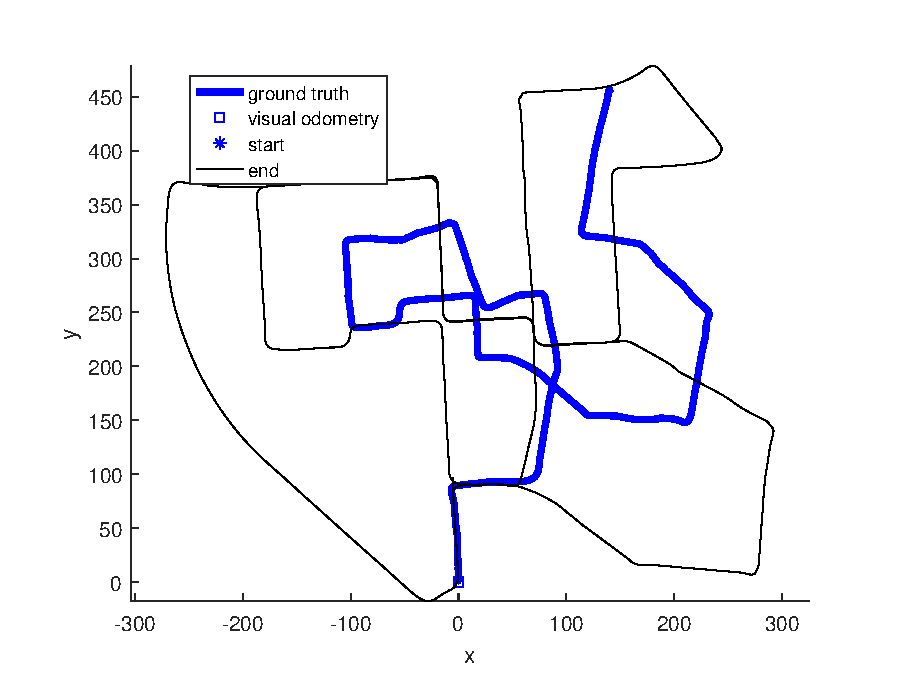
\includegraphics[height=2.7in]{results/trajectory_kitti.eps}
        \caption{Trajectory vs. ground truth}
    \end{subfigure}%
    ~ 
    \begin{subfigure}[t]{0.5\textwidth}
        \centering
        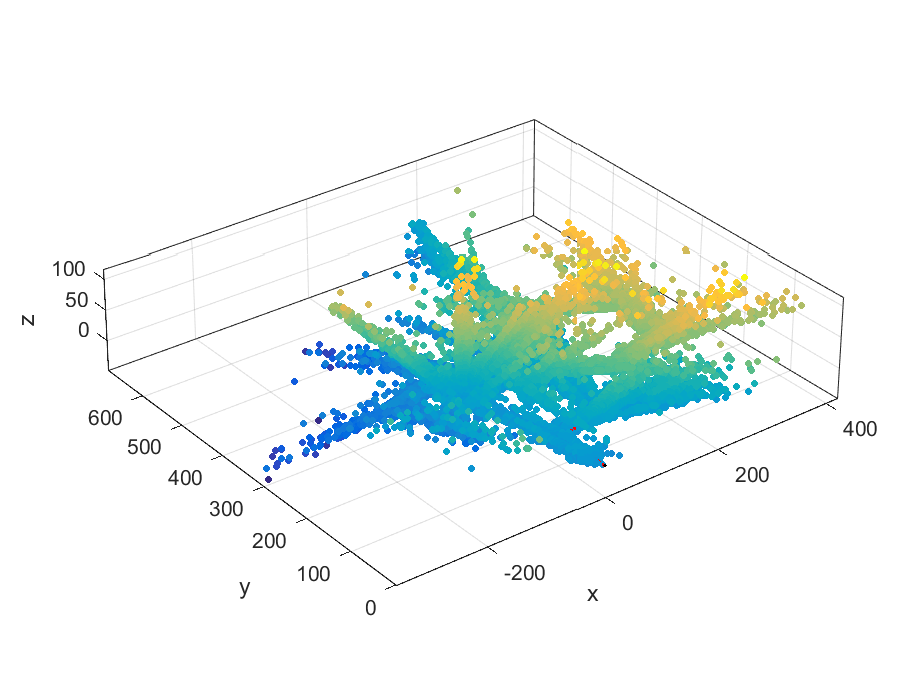
\includegraphics[height=2.7in]{results/landmarks_kitti.eps}
        \caption{3D landmarks}
    \end{subfigure}
    \caption{Kitti Dataset Results}
		\label{parking_result_fig}
\end{figure*}

\textbf{Malaga}
\begin{figure*}[ht!]
    \centering
    \begin{subfigure}[t]{0.5\textwidth}
        \centering
        \includegraphics[height=2.7in]{results/Comparison_GT_Malaga.png}
        \caption{Trajectory vs. ground truth}
    \end{subfigure}%
    ~ 
    \begin{subfigure}[t]{0.5\textwidth}
        \centering
        \includegraphics[height=2.7in]{results/Map_LM_Malaga.png}
        \caption{3D landmarks}
    \end{subfigure}
    \caption{Malaga dataset results}
		\label{parking_result_fig}
\end{figure*}

\textbf{Parking}
\begin{figure*}[ht!]
    \centering
    \begin{subfigure}[t]{0.5\textwidth}
        \centering
        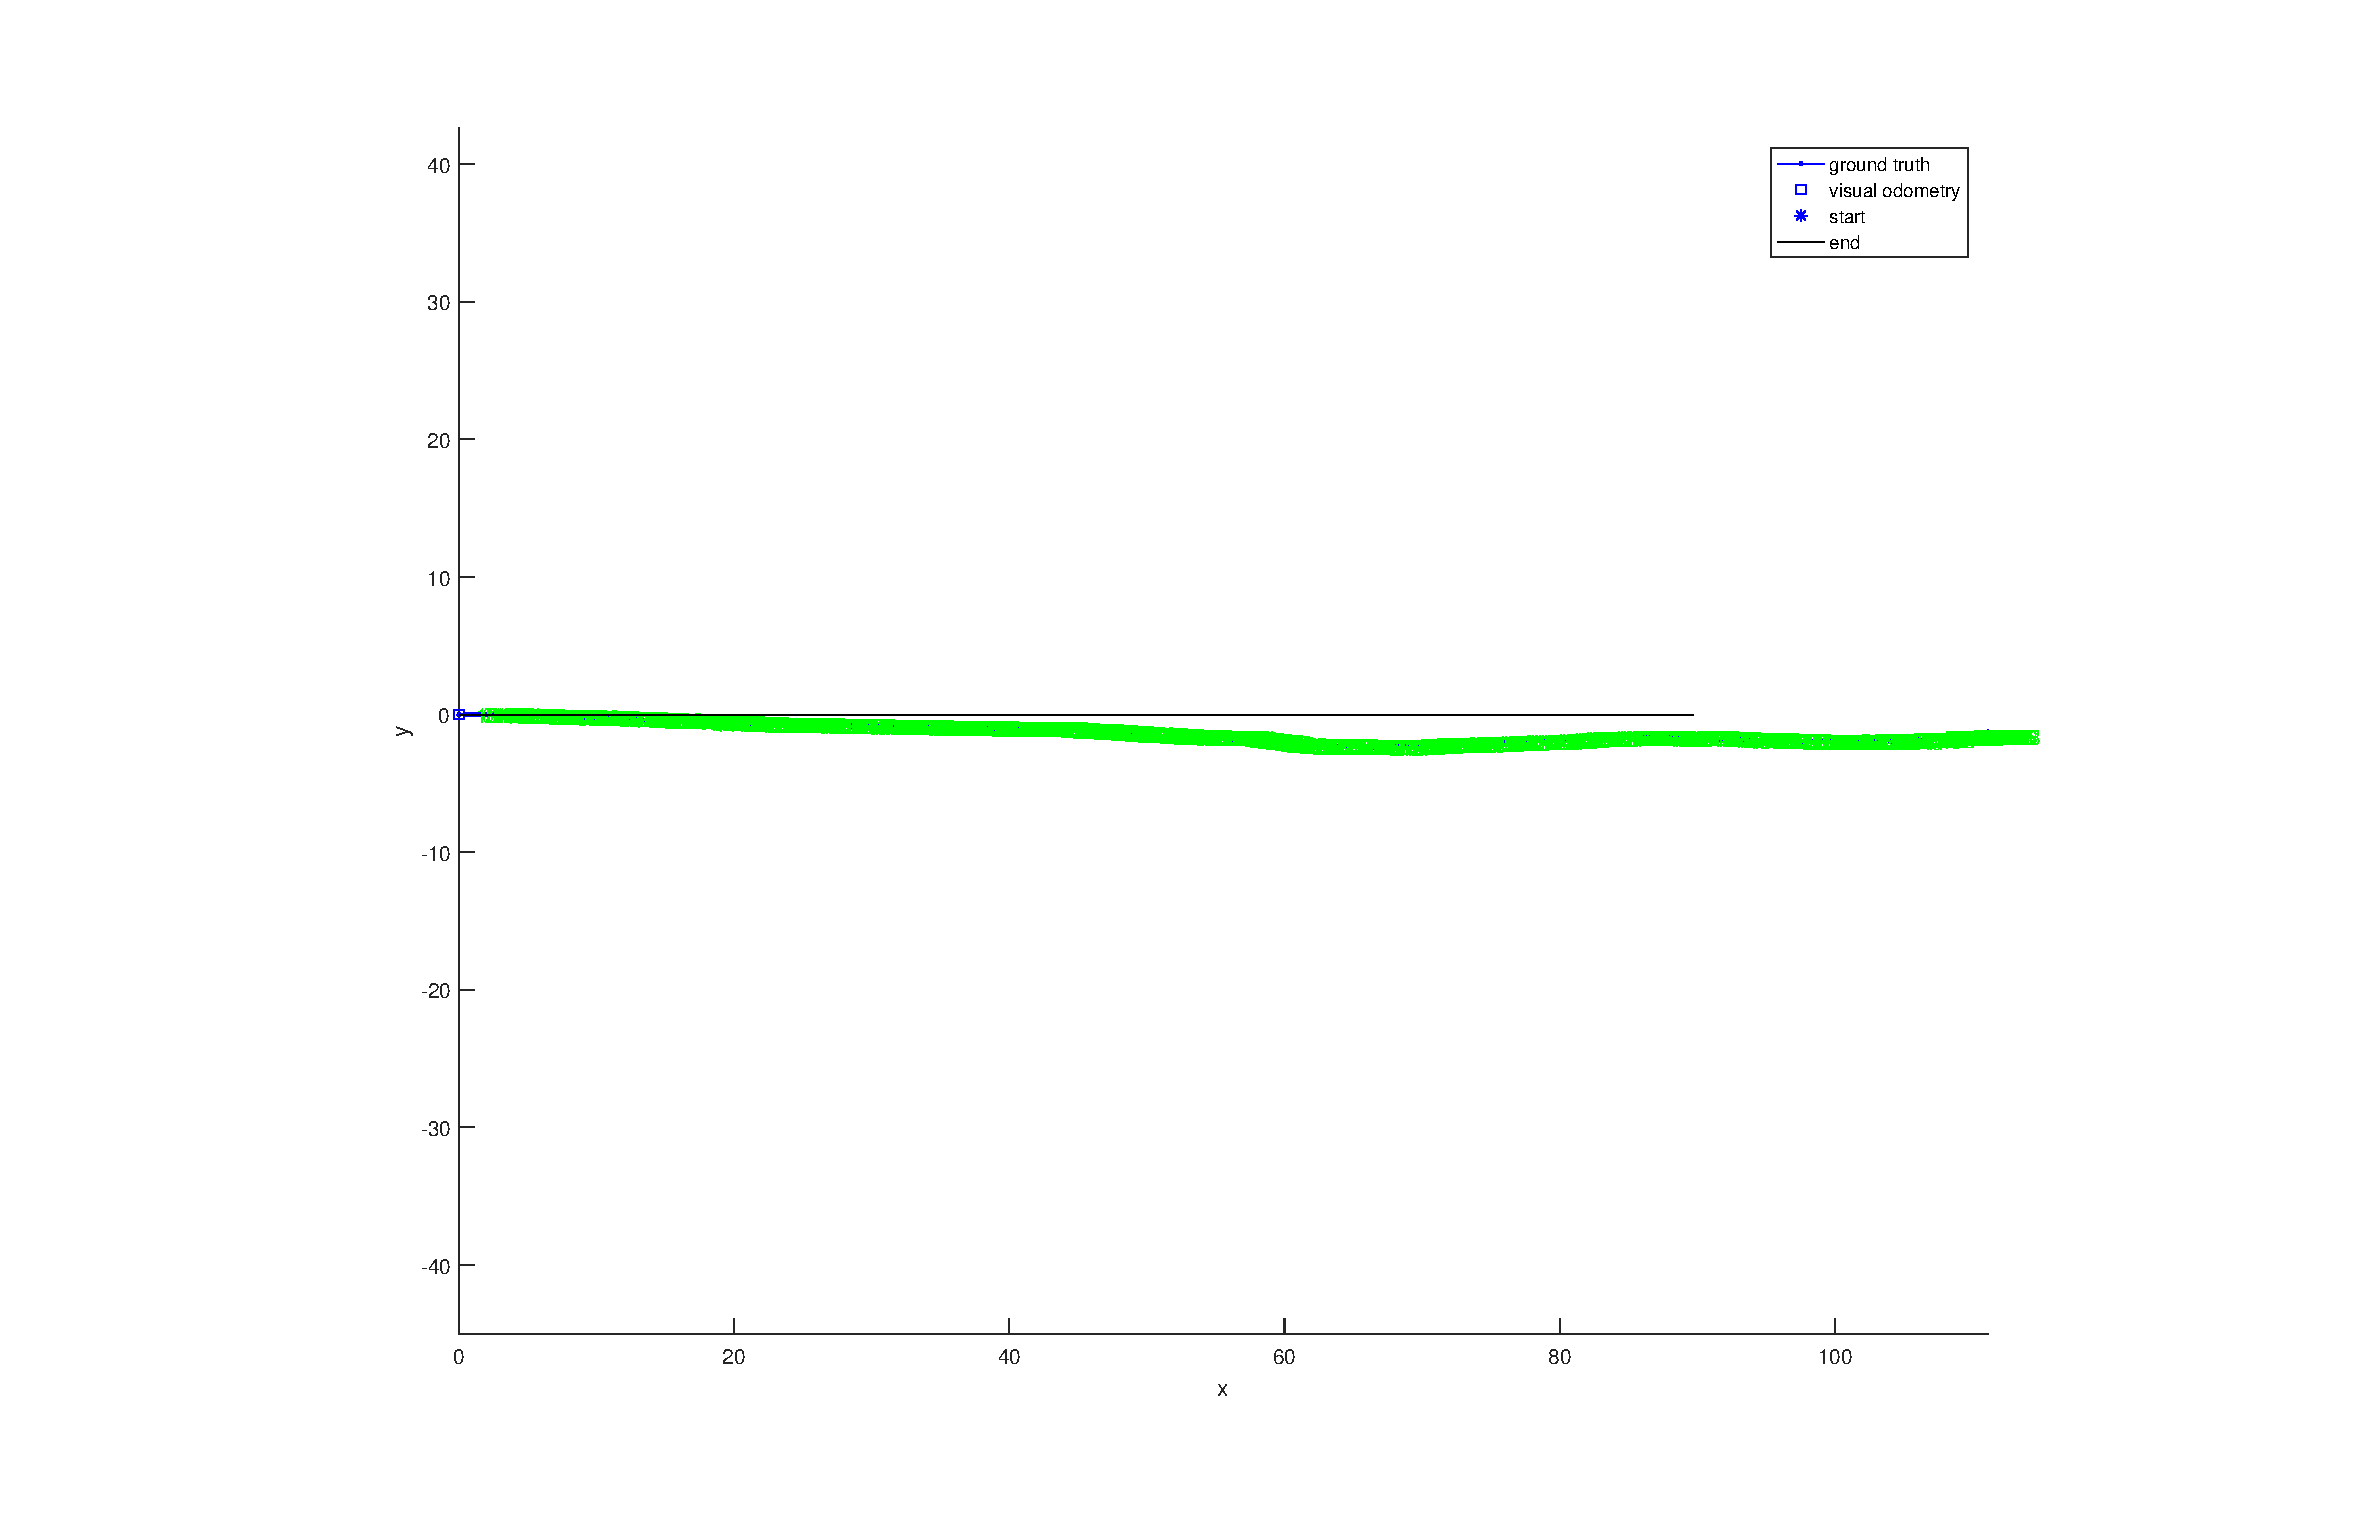
\includegraphics[height=2.7in]{results/trajectory_parking.eps}
        \caption{Trajectory vs. ground truth}
    \end{subfigure}%
    ~ 
    \begin{subfigure}[t]{0.5\textwidth}
        \centering
        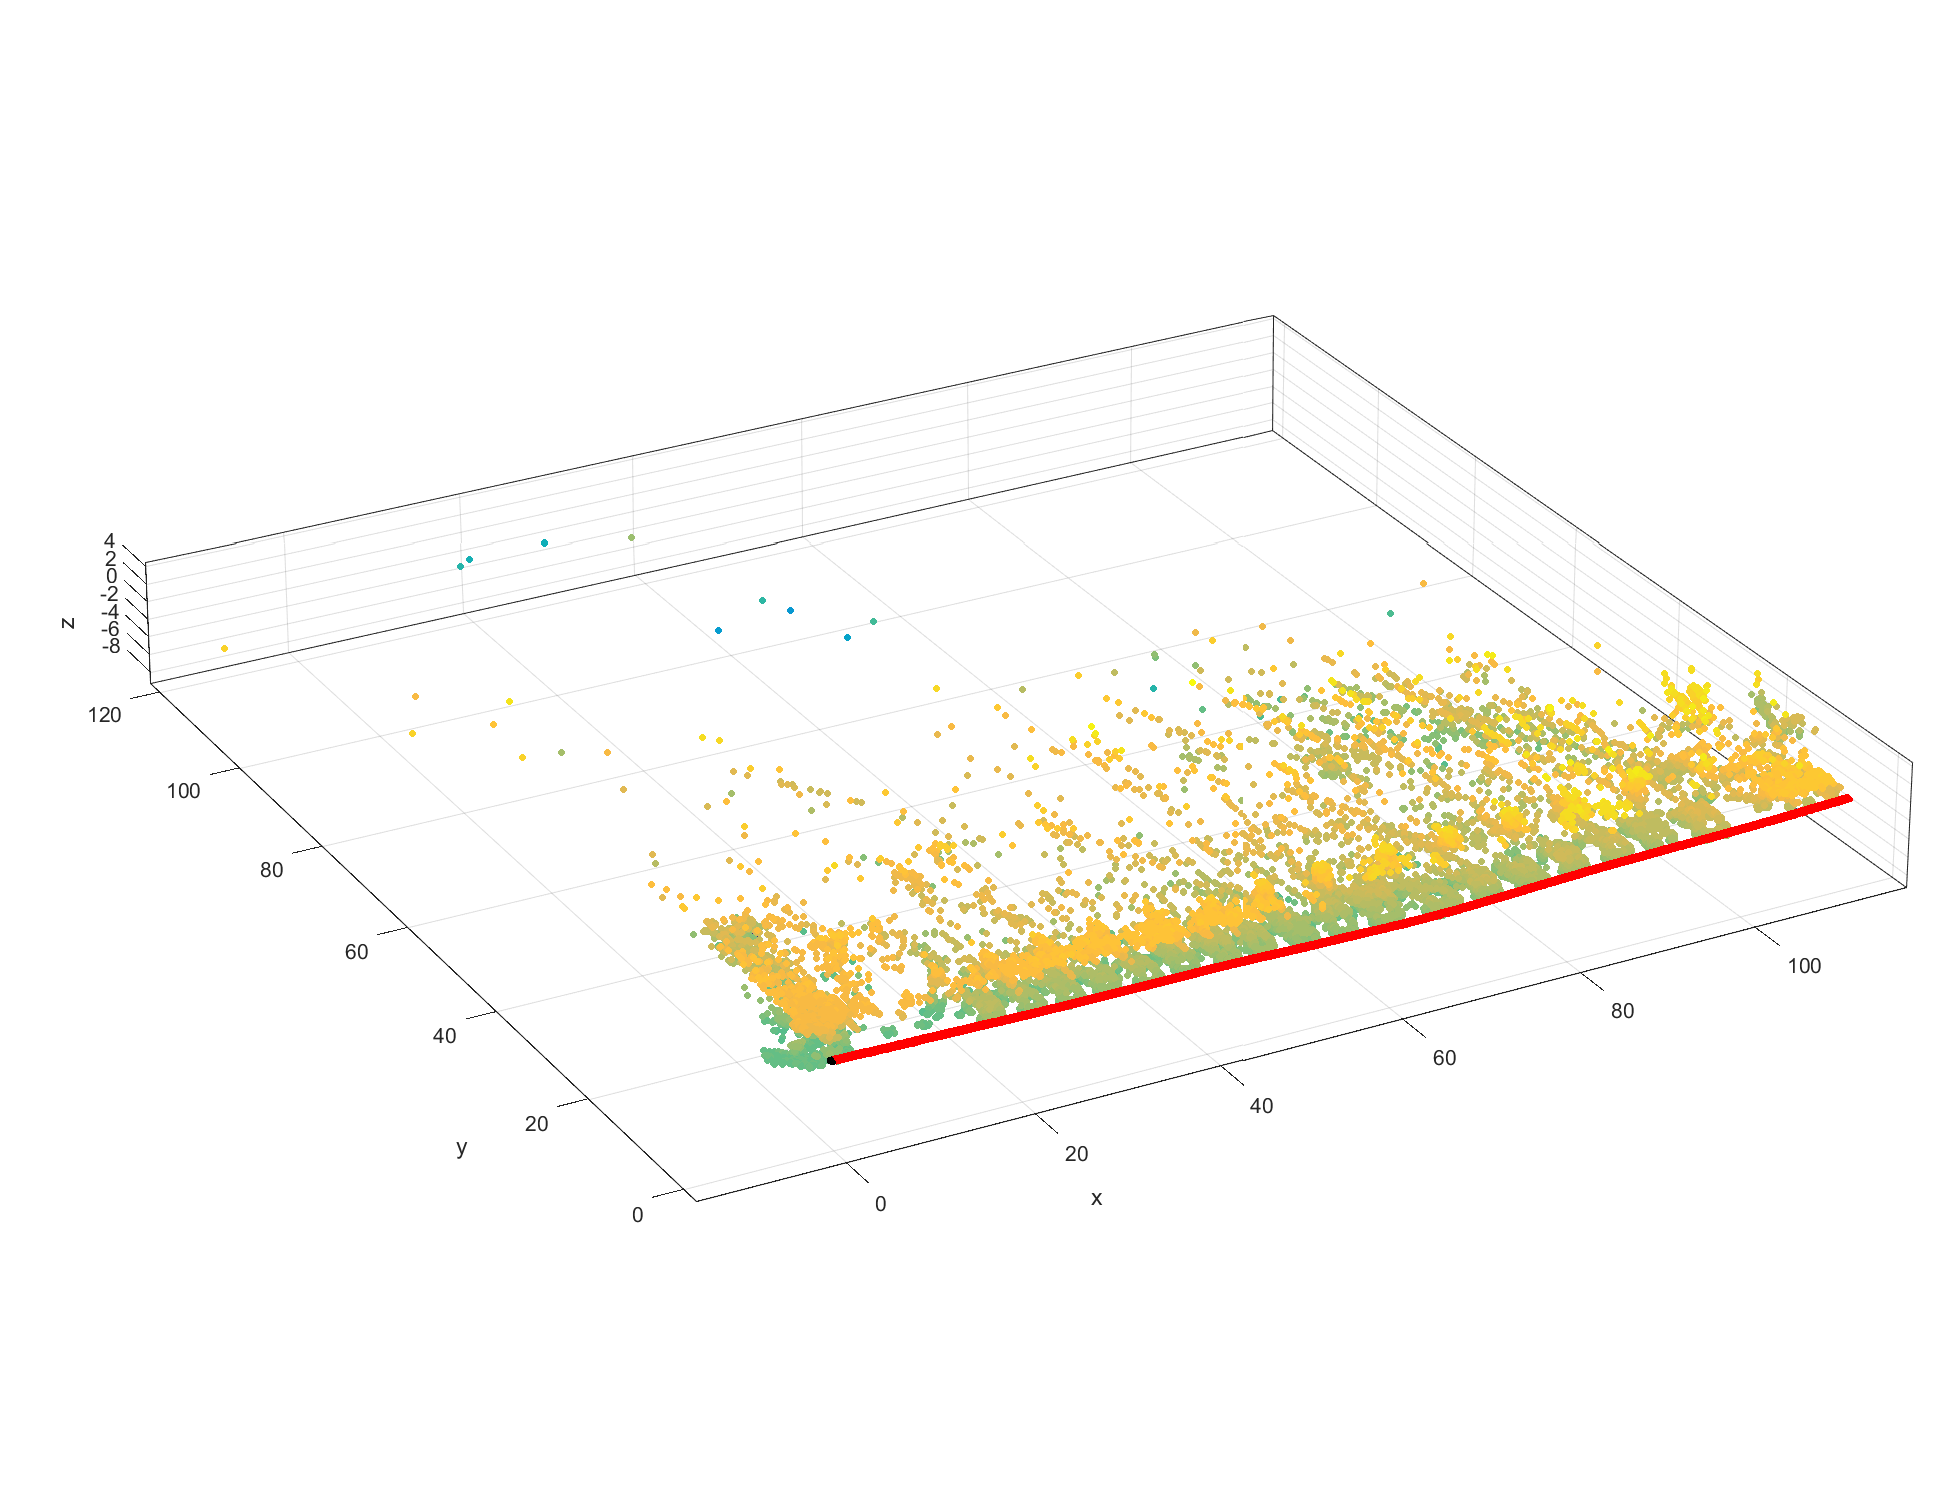
\includegraphics[height=2.7in]{results/landmarks_parking.eps}
        \caption{3D landmarks}
    \end{subfigure}
    \caption{Parking dataset results}
		\label{parking_result_fig}
\end{figure*}

\textbf{Poly Up}

\textbf{Poly Down}

\subsubsection{Speed \& Real-Timeness}
A lot of effort was invested into efficient programming (e.g. avoiding for-loops in Matlab). The parameter with the biggest impact on the frame rate was the number of iterations for the P3P-RANSAC (a classical for-loop). The frame rate depends almost linearly on this parameter. Further the more landmarks and candidate keypoints tracked the slower the pipeline. However, we preferred to generate more landmarks over having a faster pipeline in order to increase robustness and accuracy.\\

A profiling run with the Matlab profiler tool showed that most of the computational resources is spent in the following three functions in descendant order (self-time): \code{p3p()}, \code{selectKeypoints()} and \code{harris()}. The frame rates were obtained with a Core-i7 (3.5GHz) processor.

